\documentclass{article}

% packages
\usepackage[a4paper, margin=2.2cm]{geometry}
\usepackage{multicol}
\usepackage[utf8]{inputenc}
\usepackage[english]{babel}
\usepackage{minted}
\usepackage{tikz}
\usepackage{pgfplots}
\usepackage{parskip}
\usepackage{amsmath}
\usepackage{xcolor}
\usepackage[justification=centering, margin=1.6cm]{caption}
\usepackage{graphics}

\pgfplotsset{compat=1.16}

\newlength\figurewidth
\newlength\figureheight
\setlength\figurewidth{0.4\textwidth}
\setlength\figureheight{0.4\textwidth}

\begin{document}

    \begin{titlepage}
        \begin{center}
            \vspace*{2cm}
            
            {\huge \textbf{xCore-200 Cellular Automaton Farm}}
            
            \vspace{0.5cm}
            
            {\Large COMS20001 Concurrent Computing CW1}
            
            \vspace{0.5cm}
            
            {\large Team 6}
            
            \vspace{1cm}
            
            \hspace*{1cm} {\Large \textbf{Ruairi Fox}} \hfill {\Large \textbf{Liam Dalgarno}} \hspace*{1cm} \\~\\[-0.5em]
            \hspace*{1cm} MEng. Computer Science \hfill MEng. Computer Science  \hspace*{1cm} \\~\\[-1em]
            \hspace*{1cm} rf17160@bristol.ac.uk  \hfill ld17285@bristol.ac.uk  \hspace*{1cm} 
            
            \vspace{1cm}
            
            {\large \today}
        \end{center}
    \end{titlepage}

    \section{Functionality and Design}
    \subsection{Design Overview}
    To implement Conway's game of life, one of the first design decision we had was to split the board's rows between the workers. If we had two workers and 16 rows then each worker would get 8 rows. This does not actually work though as each worker needs information from the rows directly above and below it's block. To do this, we have the workers each send their redundant rows to each other, so the distributor does not store the board at all. In order to make sure that exporting arrives in the correct order, we have the distributor send a flag to the workers who will then send their portion of the board only when they have the flag. They then return the flag afterwards so that another worker can send their data. We would have had a direct channel between the workers and the data\_out but we are restricted by the hard limits of channels imposed by the board. 
    \subsection{Bit packing}
    During the program we pack 32 uchars into a single Int value allowing us to transfer the data far more quickly across channels. As well as this, The reduced size means that it is actually possible to keep the larger images on the board and process them, as without packing we would run out of space.
    \subsection{Operating in place}
    Rather than unpacking our data we decided to operate on it in place. This helps us avoid the memory and CPU overhead of packing and unpacking the data each time. During computation each processed row overwrites the row above it's original position, as that row is no longer needed for processing. This means we do not need to allocate another array to hold the results of processing.

    \begin{figure}[h]
        \begin{center}
            \begin{minted}[fontsize=\footnotesize]{C}
// l, c, r represent the shifts to get the neighbouring cell bits
// l_pack and r_pack are the left and right packed bits
// they're usually the same unless the current bit is on the edge of the pack
unsigned char l = mod(-i, 32), c = 31 - i, r = i == 31 ? 31 : 30 - i;
unsigned char l_pack = i == 0 ? mod(x - 1, PACKED_WD) : x;
unsigned char r_pack = i == 31 ? mod(x + 1, PACKED_WD) : x;
unsigned char neighbours = ((cells[u_row][l_pack] >> l) & 0x1) 
                         + ((cells[u_row][x]      >> c) & 0x1) 
                         + ((cells[u_row][r_pack] >> r) & 0x1)
                         + ((cells[y][l_pack]     >> l) & 0x1)
                         + ((cells[y][r_pack]     >> r) & 0x1)
                         + ((cells[d_row][l_pack] >> l) & 0x1) 
                         + ((cells[d_row][x]      >> c) & 0x1) 
                         + ((cells[d_row][r_pack] >> r) & 0x1);
\end{minted}
            \caption{Code that will allow the system to operate in place. }
            \label{fig:inplace}
        \end{center}
    \end{figure}
    
    
    \subsection{Concurrent Workers}
    Our program implements multiple concurrent threads working in parallel. The distributor sends the worker threads a portion of the board initially after which the workers communicate amongst themselves to transfer redundant rows.
    \subsection{Top and bottom}
    As the workers communicate between themselves for redundant rows there is potential for a deadlock if the order of sending is not well defined. Because of this, We pass a flag into each worker that defines if they send first (top) or receive first (bottom). This  allows us to concurrently send the ghost rows between threads.


    \newpage
    \section{Tests and Experiments}
    
    We tested our system in multiple ways, such as:
    
    \begin{itemize}
        \setlength\itemsep{-0.2\baselineskip}
        \item Comparing two iterations of a \verb|32x32| image to another implementation of the Game of Life. (Figure \ref{fig:test32})
        \item Testing the example \verb|512x512| image given (Figure \ref{fig:testexamples})
        \item Examining some sample generations of a \verb|1024x1024| image starting from a straight line. (Figure \ref{fig:test1024})
        \item Varying the worker count and image size. (Section \ref{workercount})
        \item Changing the distribution of workers across the tiles. (Section \ref{workerdistribution})
    \end{itemize}
    
    \begin{figure}[h]
        \begin{center}
            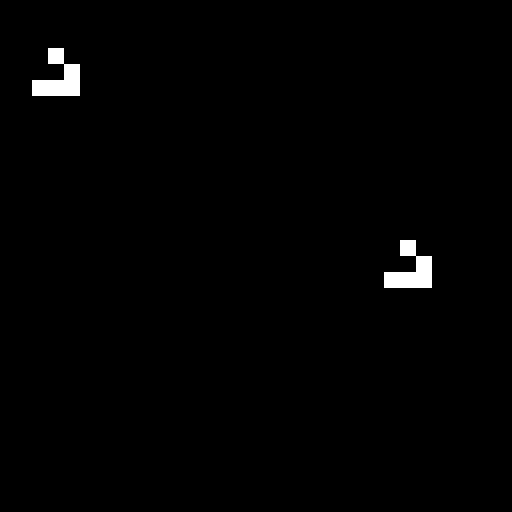
\includegraphics[width=0.15\textwidth]{test32.png}
            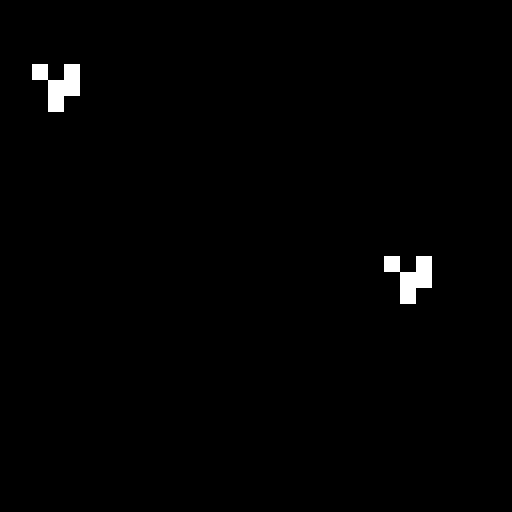
\includegraphics[width=0.15\textwidth]{testout32-1.png}
            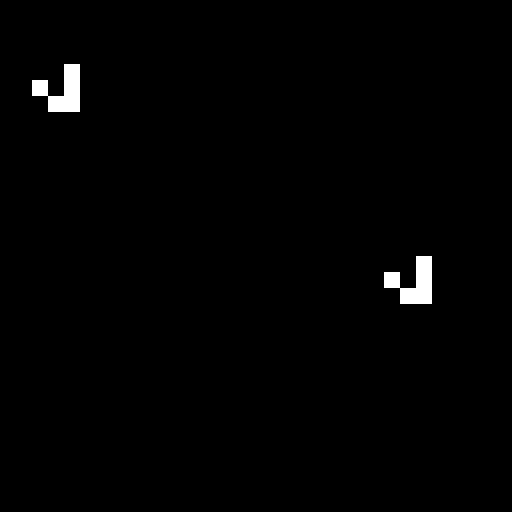
\includegraphics[width=0.15\textwidth]{testout32-2.png}
            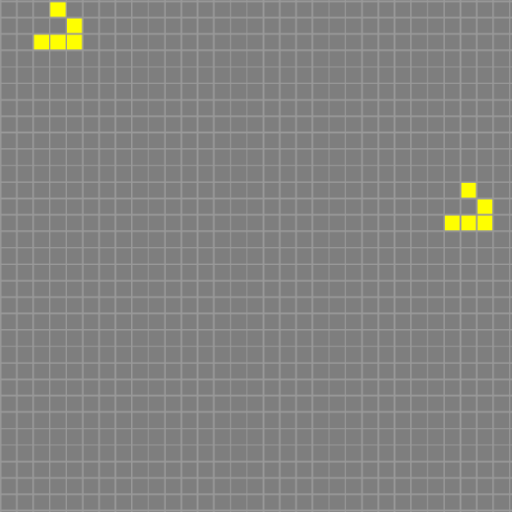
\includegraphics[width=0.15\textwidth]{verify32.png}
            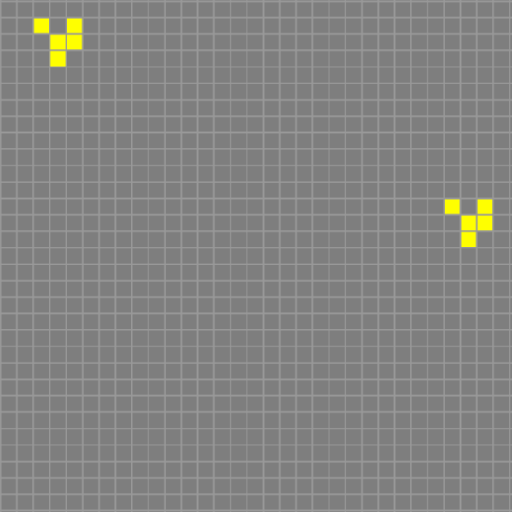
\includegraphics[width=0.15\textwidth]{verify32-1.png}
            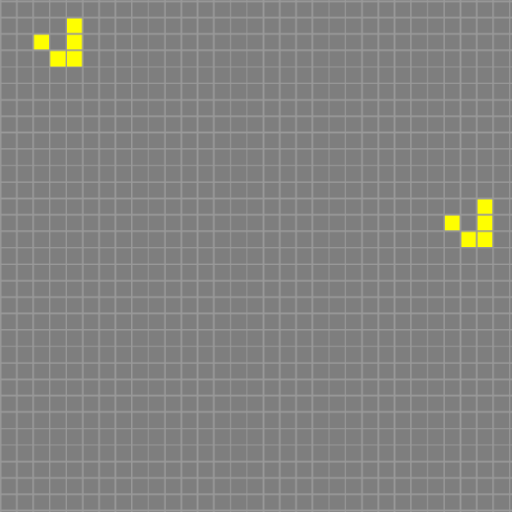
\includegraphics[width=0.15\textwidth]{verify32-2.png}
            \caption{State following 2 iterations of a \texttt{32x32} image. \\ Left: our system; Right: \texttt{https://bitstorm.org/gameoflife/}}
            \label{fig:test32}
        \end{center}
    \end{figure}

    \begin{figure}[h]
        \begin{center}
            
\includegraphics[width=0.15\textwidth]{test256.png}
            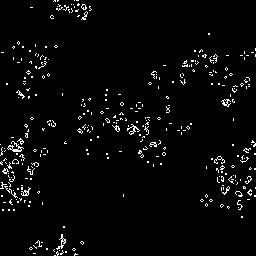
\includegraphics[width=0.15\textwidth]{testout256.png}
            \caption{The state of \texttt{256x256} following 100 iterations.}
            \label{fig:test256}
        \end{center}
    \end{figure}

    \begin{figure}[h]
        \begin{center}
            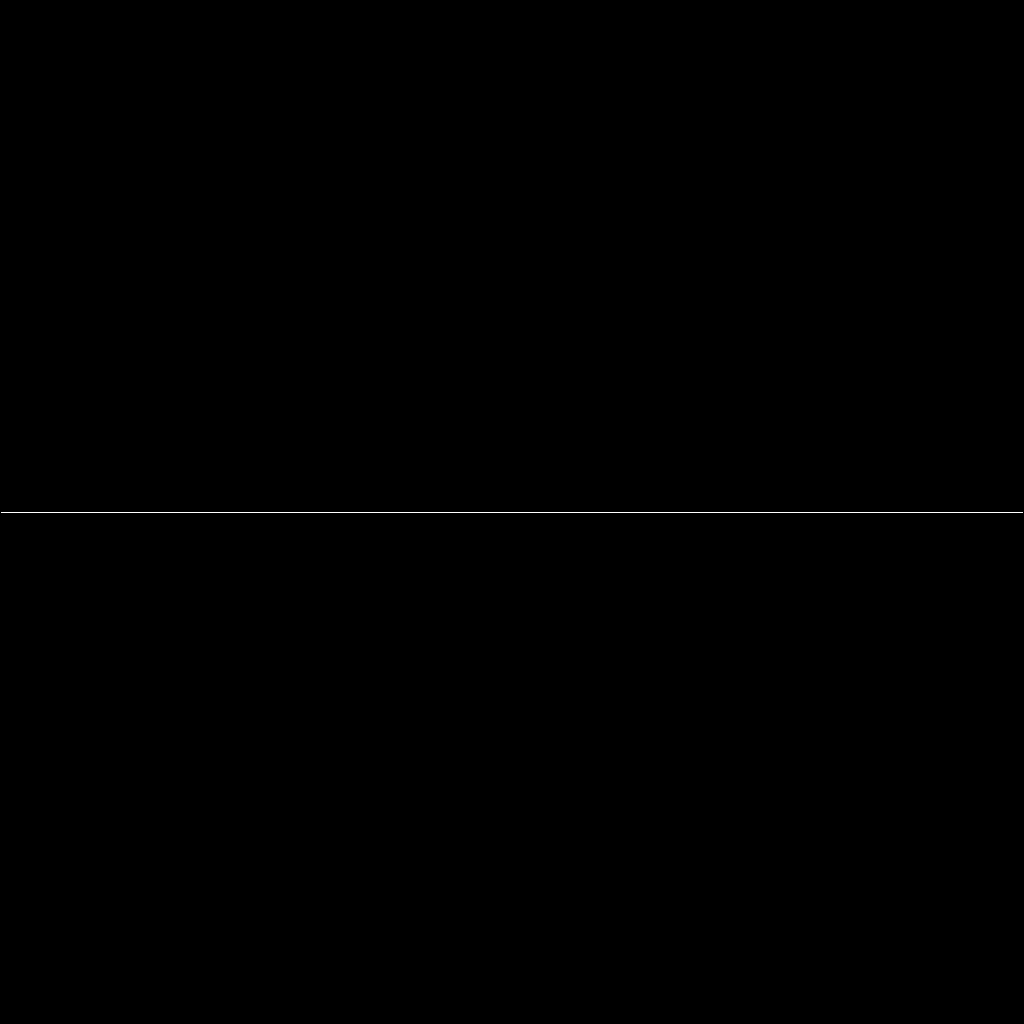
\includegraphics[width=0.2\textwidth]{test1024.png}
            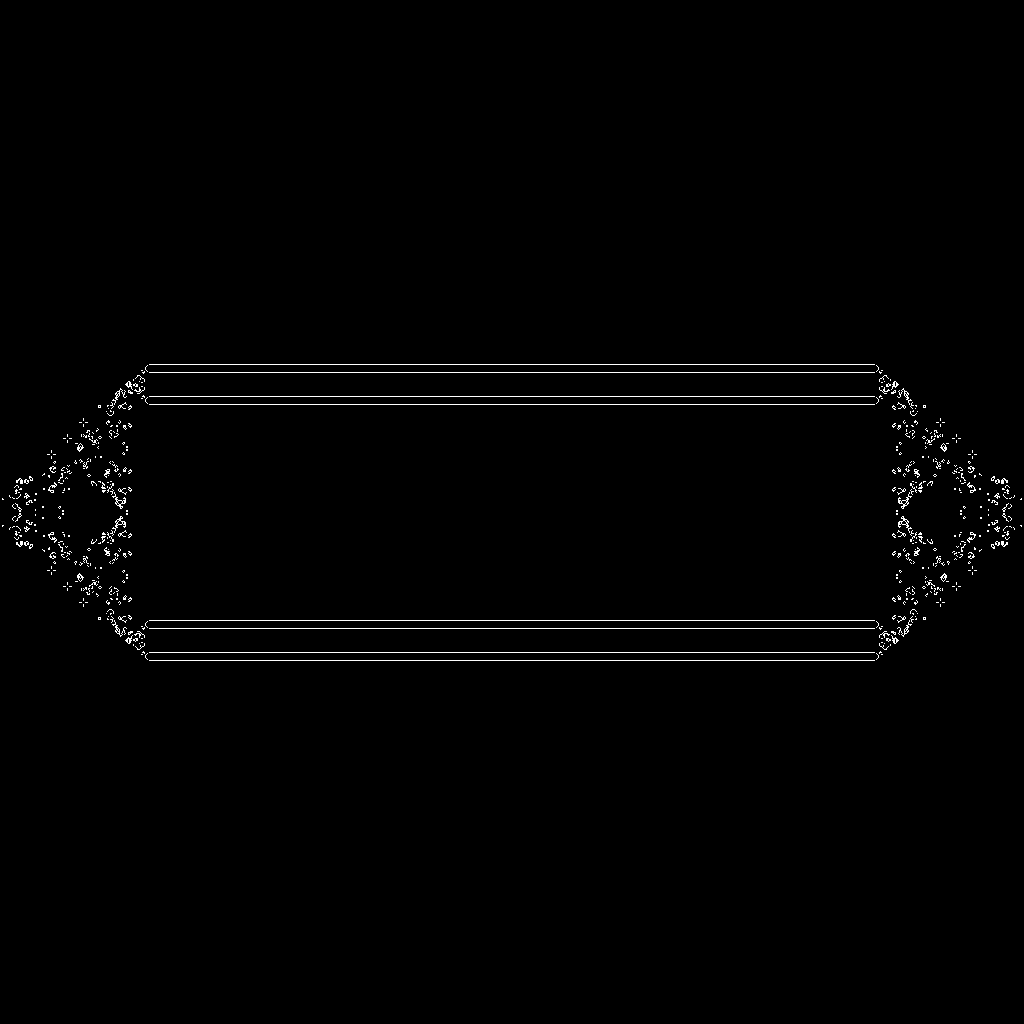
\includegraphics[width=0.2\textwidth]{testout1024-1.png}
            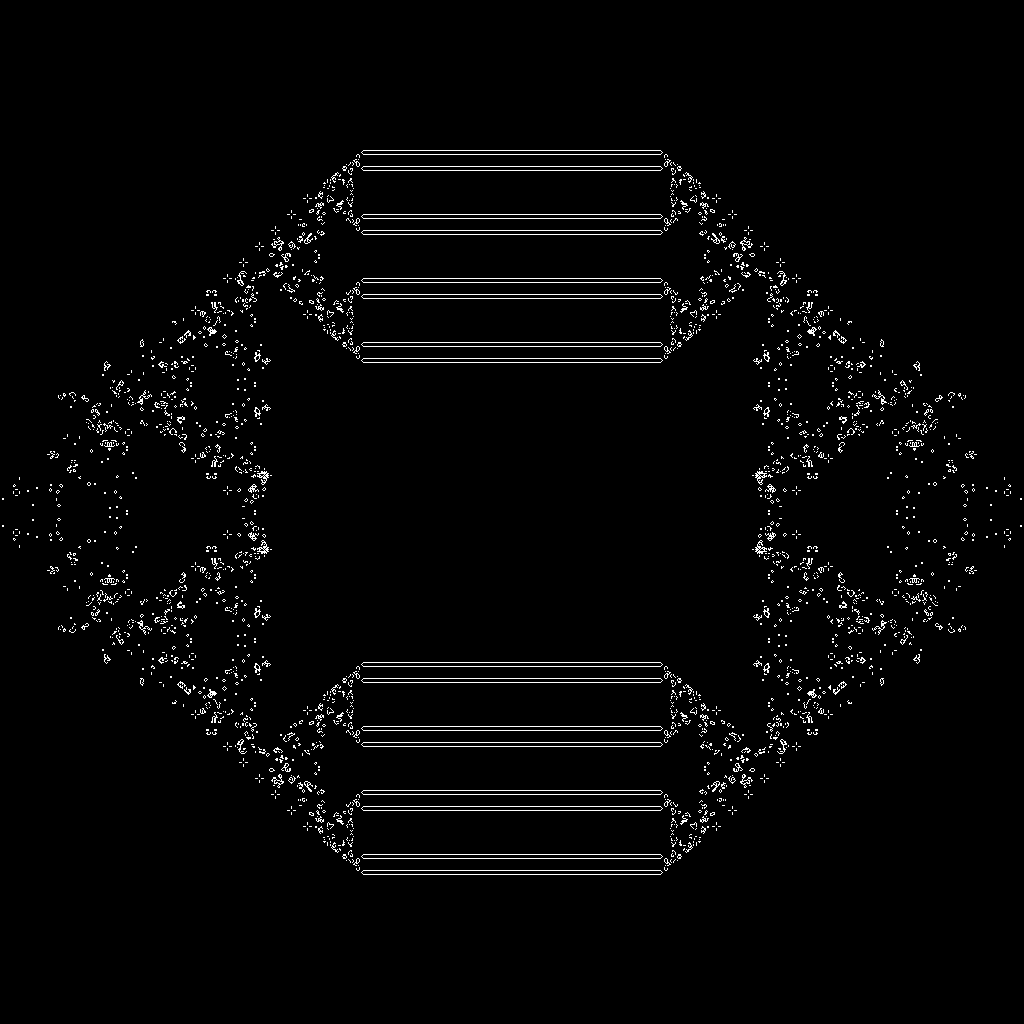
\includegraphics[width=0.2\textwidth]{testout1024-2.png}
            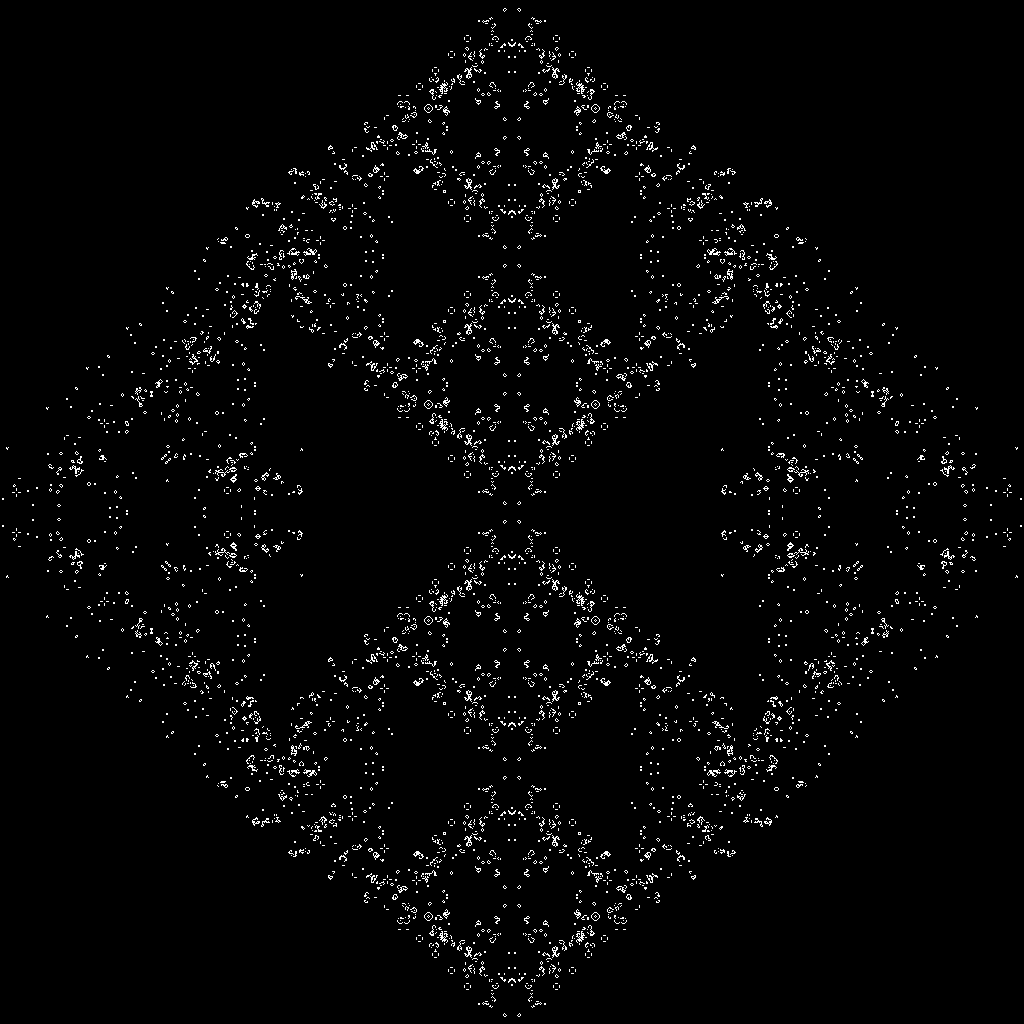
\includegraphics[width=0.2\textwidth]{testout1024-3.png}
            \caption{Example generations of a \texttt{1024x1024} image, beginning from a straight line.}
            \label{fig:test1024}
        \end{center}
    \end{figure}
    
    \subsection{Worker Count} 
    \label{workercount}

    \begin{figure}[h]
        \begin{center}
            {\small
\begin{tabular}{|c|c|c|c|c|}
    \hline Size & AGT2 (ms) & AGT4 (ms) & AGT8 (ms) \\
    \hline \verb|64x64| & 11.64 & 11.65 & 11.64 \\
    \verb|128x128| & 39.88 & 20.12 & 11.64 \\
    \verb|256x256| & 161.89 & 80.77 & 40.31 \\
    \verb|512x512| & 621.29 & 313.71 & 157.88 \\
    \verb|1024x1024| & 2472.33 & 1250.44 & 622.59 \\
    \hline
\end{tabular}}
            \caption{The effect of increasing worker count and size of image on Average Generation Time.}
            \label{fig:agt}
        \end{center}
    \end{figure}
    
    \begin{figure}[h]
        \begin{center}
            % This file was created by matplotlib2tikz v0.6.18.
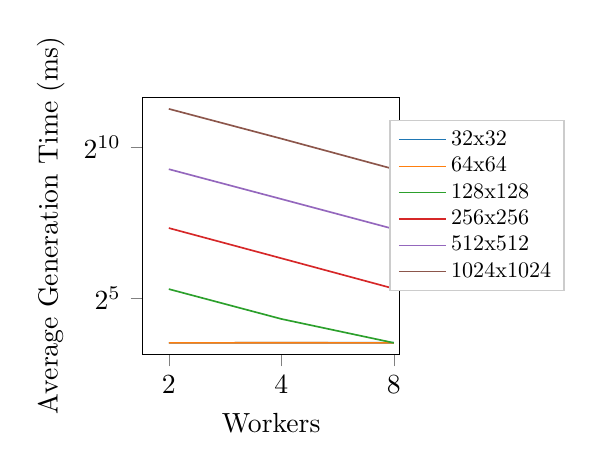
\begin{tikzpicture}

\definecolor{color0}{rgb}{0.12156862745098,0.466666666666667,0.705882352941177}
\definecolor{color1}{rgb}{1,0.498039215686275,0.0549019607843137}
\definecolor{color2}{rgb}{0.172549019607843,0.627450980392157,0.172549019607843}
\definecolor{color3}{rgb}{0.83921568627451,0.152941176470588,0.156862745098039}
\definecolor{color4}{rgb}{0.580392156862745,0.403921568627451,0.741176470588235}
\definecolor{color5}{rgb}{0.549019607843137,0.337254901960784,0.294117647058824}

\begin{axis}[
height=\figureheight,
legend cell align={left},
legend entries={{32x32},{64x64},{128x128},{256x256},{512x512},{1024x1024}},
legend style={nodes={scale=0.8, transform shape}, at={(1.3,0.91)}, anchor=north, draw=white!80.0!black},
tick align=outside,
tick pos=left,
width=\figurewidth,
x grid style={white!69.01960784313725!black},
xlabel={Workers},
xmin=1.7, xmax=8.3,
y grid style={white!69.01960784313725!black},
ylabel={Average Generation Time (ms)},
ymin=8.90420822429587, ymax=3231.94611750847,
ymode=log,
xmode=log,
log basis x={2},
log basis y={2},
xticklabel=\pgfmathparse{2^\tick}\pgfmathprintnumber{\pgfmathresult}
]
\addlegendimage{no markers, color0}
\addlegendimage{no markers, color1}
\addlegendimage{no markers, color2}
\addlegendimage{no markers, color3}
\addlegendimage{no markers, color4}
\addlegendimage{no markers, color5}
\addplot [semithick, color0]
table [row sep=\\]{%
2	11.64 \\
4	11.65 \\
8	11.66 \\
};
\addplot [semithick, color1]
table [row sep=\\]{%
2	11.64 \\
4	11.65 \\
8	11.64 \\
};
\addplot [semithick, color2]
table [row sep=\\]{%
2	39.88 \\
4	20.12 \\
8	11.64 \\
};
\addplot [semithick, color3]
table [row sep=\\]{%
2	161.39 \\
4	80.77 \\
8	40.31 \\
};
\addplot [semithick, color4]
table [row sep=\\]{%
2	621.29 \\
4	313.71 \\
8	157.88 \\
};
\addplot [semithick, color5]
table [row sep=\\]{%
2	2472.33 \\
4	1250.44 \\
8	622.59 \\
};
\end{axis}

\end{tikzpicture}
            \caption{Log plot of Average Generation Time vs. Worker Count.}
            \label{fig:agtplot}
        \end{center}
    \end{figure}

    We can measure the processing speed by the AGT (Average Generation Time). From Figure \ref{fig:agt} it's clear that increasing the number of workers is effective at reducing the AGT. Originally, we had a bottleneck which caused the AGT to not go any lower than 11.64ms, regardless of worker count. We pinpointed the cause as the accelerometer, as each time the distributor requested the most recent accelerometer data, it had to wait for the thread to read from the register. 
    
    Instead, we added another thread which holds the most recent accelerometer data when available and passes it to the distributor when requested. We did encounter a bug in the system, so we decided to exclude this fix from the stable submitted version. The data in Figure \ref{fig:agt} is from the patched version.

    Following the fix, doubling the worker count halves the AGT, which implies that increasing the workers gives a \textit{linear} speed up, and this is reflected by the straight lines in Figure \ref{fig:agtplot}. Furthermore, increasing the image size by a factor of 4 also increases the AGT by a factor of 4; this is expected since an $n$-fold increase in the number of cells is an $n$-fold increase in the amount of work. A nice consequence of this behaviour is that the AGT of an image with $n$ cells and $m$ workers is approximately the same as the AGT of an image with $4n$ cells and $4m$ workers (e.g. the AGT of \verb|128x128| with 2 workers is approximately equal to the AGT of \verb|256x256| with 8 workers).

    \subsection{Worker Distribution} 
    \label{workerdistribution}

    In the \verb|xCore-200| there are \textbf{hard} and \textbf{soft} channels, where hard channels are across physical tiles, and soft channels are between individual threads on a tile. Hard channels will have higher latency since the data must travel a larger distance in comparison to a soft channel. We can vary the number of hard channels by either changing the position of the distributor with respect to the tiles: if they're on separate tiles then there'll be more hard channels.

    In our experiment we tested the distributor position using 4 workers (as we cannot have more than 8 threads on a single tile), and the worker distribution using both 8 and 4 workers.

    \begin{figure}[h]
        \begin{center}
            {\footnotesize
% add varying worker count
\begin{tabular}{|c|c|c|}
    \hline Size & Distribution & AGT (ms) \\
    \hline \verb|256x256| & Same tile & 80.2 \\
    \verb|256x256| & Different tiles & 81.37 \\
    \verb|256x256| & Split across both tiles & 80.78 \\
    \hline \verb|512x512| & Same tile & 314.47 \\
    \verb|512x512| & Different tiles & 311.7 \\
    \verb|512x512| & Split across both tiles & 313.7 \\
    \hline
\end{tabular}}
            \caption{Varying the communication channels between the distributor and workers.}
            \label{fig:distribution}
        \end{center}
    \end{figure}

    However, the data suggests that changing the organisation of the distributor and workers does not affect the AGT, and there seems to be no trend between results. This implies that the communication is not limiting the AGT. It is still best to store the workers across both tiles, as (especially for 8 workers) the memory is shared equally and we can make use of the full 512KB of RAM. 
    
    \pagebreak

    % ?? is a placeholder for a future citation :)
    \section{Critical Analysis} 
    \label{analysis}

    The maximum size that our image can process is \verb|1792x1792| which is 3,211,264 cells, using up to 8 workers. Figure \ref{fig:agt} shows how fast our system can evolve from \verb|32x32| to \verb|1024x1024| with a varying amount of workers. Although we have solved many problems to increase the maximum image size, we could go further. 

    \subsection{Limiting Factors} \label{limits}

    A large limiting factor of our program is that it cannot process images which do not have a width which is a multiple of 32. This is a result of our packing algorithm and evolution algorithm, which both rely on there being 32 full bits to work correctly. Instead we could implement a fallback strategy, such as packing into smaller packets so that more sizes are supported.

    Our system also does not work with only a single worker. It relies on a worker having two neighbours so that they can be connected together through channels. Ideally, we could dynamically choose a strategy depending on how many workers there are, e.g. if there is a single worker, then don't run concurrently and rely on having neighbours.

    \verb|data_in| and \verb|data_out| read/write to the file one line at a time. For an image with width $w$ this wastes $2w$ bytes, as both the \verb|data_in| and \verb|data_out| must preallocate $w$ bytes for the line. Instead, we could read/write to the file a packet at a time, which means that only 4 bytes would be allocated for each.

    Currently, the distributor acts as a controller which coordinates other tasks such as exporting, timing, initialisation etc. It is connected to every worker so that it can notify them when to export. However, we could change the first worker to be a `master' worker which communicates with the distributor and cascades the messages to the other workers. This would remove the need for each worker to be connected to the distributor, and we could therefore connect each worker directly to \verb|data_out| to avoid the distributor becoming a bottleneck. 

    \subsection{Future Considerations}
    
    We did not have the chance to test how using asynchronous channels impacts the performance compared to synchronous channels. Asynchronous channels operate using a buffer which may prove useful when the workers need to swap their overlapping rows: a worker can simply place the data on the buffer even if the receiver is currently busy (assuming the buffer is not full).

    Additionally, the \verb|xCore-200| is harshly limited by its I/O speed, with larger boards taking upwards of 10 minutes to transfer to/from the board. We could dynamically generate the image on the board to skip transfer times, and also generate known patterns/structures to allow for easier testing.

    We could connect multiple \verb|xCore-200| boards together and implement cross-board communication. This would enable us to use more workers, channels, and memory which would massively increase the maximum board size. Communication across the boards would be quite slow however since the packets have a larger distance to travel and therefore larger latency.

    Currently, the program stores every single cell but packed into a \verb|uint32|. Instead, we could identify common `structures' that occur within the Game of Life, such as lengths of dead cells or gliders, and give them some sort of identifier. This would allow the program to skip over large sections of dead cells as they will not be alive in the next generation, or to swap out known structures easily as we know how they progress. 
    
    A much more difficult yet rewarding evolution strategy would be that of HashLife, which is able to optimise the rules of the Game of Life and remove redundancy. Unfortunately, HashLife is implemented using a \verb|quadtree| and is also memoized (i.e. it stores the results of previous computations). These two factors together mean that although it was significant gains in performance, it also has significant gains in memory usage, which may not be viable for large board sizes on the \verb|xCore-200|. On the other hand, it may be exceptional at evolving smaller board sizes where memory is less of an issue.

\end{document}